%----------------------------------------------------------------------------------------
\chapter{Background}
\label{chap:background}
%----------------------------------------------------------------------------------------
This chapter describes the two main driving factors for a complete re-design of ScaFi, which are the \ac{XC} and Scala 3.
%
On one hand, \ac{XC} opens the way for considerable design improvements given the simpler set of foundational constructs it requires, consisting of the single primitive \texttt{exchange}, from which the entire language takes its name.
%
Additionally, it provides new opportunities for aggregate program developers, enabled by the expressiveness of \ac{XC}, regarding, in particular, the possibility of sending differentiated messages to neighbors using the \texttt{exchange} primitive\cite{xc}.
%
On the other hand, Scala 3 introduces significant breaking language changes and improvements from Scala 2, nevertheless featuring binary retro-compatibility.
%
This promotes the rewriting of Scala 2 libraries in a way that exploits the new language features while providing cross-builds to Scala 2 enabled by the Scala 3 compiler \quotes{Dotty}\footnote{\url{https://github.com/lampepfl/dotty}}.

\section{The Exchange Calculus}\label{chap:background->sec:xc}

\ac{XC} is a language that formalizes a tiny set of key mechanisms, sufficient to express the overall behavior of a distributed collective adaptive systems in a declarative fashion\cite{xc}.
%
\ac{XC} offers both an operational semantics, defining the local interpretation of these mechanisms on each device, and a denotational semantics, which provides an interpretation of these mechanisms at the network level, abstracting away the operational semantics details.
%
Therefore, operational semantics guides the implementation of \ac{XC} as a framework, while denotational semantics is the sole knowledge base necessary when programming a \ac{CAS} with this language.
%
The \ac{XC} language generalizes over \ac{FC} and is derived from the typed lambda calculus\cite{xc}.

The building blocks of \ac{XC} are:
\begin{itemize}
    \item the basic system model and its assumptions;
    \item the data type for neighboring values, \textit{NValues};
    \item the only communication primitive, \texttt{exchange};
    \item the concept of \textit{alignment}.
\end{itemize}

\subsection{System model}

Similarly to \ac{FC}, \ac{XC} targets a system modeled as a collection of devices, generally equipped with sensors and/or actuators, that repeatedly compute execution \textit{rounds} of the \textbf{same program} and exchange asynchronous \textit{messages} with their respective neighbors\cite{xc}.
%
In this environment, a device can fail, reboot, experience network outages, and dynamically change neighbors.
%
At each execution round, a device independently gathers a local context, consisting of inbound messages from neighbors, sensors data, and memory of its previous round of execution, if any, and then \textit{atomically executes} the \ac{XC} program common for all the devices, acting on its local context\cite{xc}.
%
The program can result in an output, that comprises side effects such as actuation, as well as, implicitly, the messages to send to neighbors for coordination\cite{xc}.
%
At the end of each round, a device begins waiting for an arbitrary time lapse, during which the device is considered \quotes{sleeping}.
%
After the sleep time, the device \quotes{wakes up} and begins the next execution round\cite{xc}.
%
During sleep, a device must still collect inbound messages and apply two policies: \textit{last-message buffering} and \textit{last-message dropping}.

\paragraph{Last-message buffering} means that every message received by a device is collected in a buffer and kept until some established criterion determines its \textit{expiration}, even across multiple execution rounds\cite{xc}.
%
As a result, the message expiration is also the minimum time that a device takes to realize that a neighbor has disappeared, either because of a failure or a neighbor network change.

\paragraph{Last-message dropping} means that every message received by a device supersedes the last message, still in the buffer, coming from the same device.\cite{xc}
%
This implies a notion of identity of devices, which is a way to recognize a neighbor's identity to discard obsolete messages coming from them.

\paragraph{Communication between devices} defined in \ac{XC} is agnostic of the message exchange medium, channel, network topology, or discovery mechanisms.
%
Messages in such a model are subject to classic distributed systems communication properties, such as unpredictable delays and drops\cite{xc}.
%
Additionally, for \ac{XC} and its implementations, a device memory of its previous execution round result can be considered a self-message at all effects.
%
This consideration models a reboot, which in practice is a memory loss, to a self-message drop, thus simplifying the device model in the operational semantics.

\subsection{NValues}

\ac{XC} features two kind of values, \textit{local values} and \textit{neighbouring values} (NValues or nvalues).
%
Local values $l$ refer to all the traditional types \texttt{A} like integer, float, list, and so on.
%
NValues, instead, are a map $\underline{\mathbf{w}}$ from device identifiers $\delta_i$ to local values $l_i$, with a default local value $l$, written $l[\delta_1 \mapsto l_1, ..., \delta_n \mapsto l_n]$\cite{xc}.

NValues refer to values coming from neighbors, which, in highly decoupled distributed systems, almost always consist of a subset of all devices, for example, because all other devices are out of reach in a spacial-dependent neighboring relationship.
%
The default value is used when evaluating a NValue $\underline{\mathbf{w}} = l[\delta_1 \mapsto l_1, ..., \delta_n \mapsto l_n]$ for a given $\delta_i$ with $\delta_i$ not present in $\underline{\mathbf{w}}$.
%
The notation above can thus be read as \quotes{the nvalue $\underline{\mathbf{w}}$ is $l$ everywhere (i.e. for all neighbors) except for devices $\delta_1, ..., \delta_n$ with values $l_1, ..., l_n$, respectively}\cite{xc}.

For example, in \Cref{fig:xc-nvalues-exampke}, the device $\delta_2$ wakes up for computation $\epsilon_2^4$ and processes a nvalue $\underline{\mathbf{w}} = 0[\delta_1 \mapsto 5, \delta_3 \mapsto 4, \delta_4 \mapsto 2]$, which corresponds to the messages carrying the scalar values 5, 4, and 2 sent by devices $\delta_1$, $\delta_3$, and $\delta_4$, respectively, some of which while device $\delta_2$ was asleep.
%
For all other devices, the entry in $\underline{\mathbf{w}}$ evaluates to $0$.
%
After the computation, $\delta_2$ sends out the messages represented by $\underline{\mathbf{w'}} = 0[\delta_1 \mapsto 7, \delta_4 \mapsto 1]$.
%
For instance, $7$ is sent to $\delta_1$, $1$ to $\delta_4$, and $0$ to all other neighbors, such as $\delta_3$.
%
Evaluation of a nvalue for a given $\delta'$ can be noted as $\underline{\mathbf{w}}(\delta')$ and its result is the local value $l'$ if $\delta' \mapsto l'$ is in $\underline{\mathbf{w}}$, or else the default value $l$ of $\underline{\mathbf{w}}$.
%
For $\underline{\mathbf{w'}}$, $\underline{\mathbf{w'}}(\delta_1)$ is $7$, and $\underline{\mathbf{w'}}(\delta_3)$ is 0.
%
Another notation used in the paper is $\underline{A}$, to indicate the type of a nvalue $\underline{\mathbf{w}} = l[\delta_1 \mapsto l_1, ..., \delta_n \mapsto l_n]$ where $l_1, ..., l_n$ are of type $A$\cite{xc}.

NValues generalize local values, in the sense that a local value $l$ with type $A$ can be automatically converted to a nvalue $l[]$ with type $\underline{A}$, with $l$ as the default value for every device\cite{xc}.
%
This simplifies the formalization of \ac{XC}, where local values and nvalues are treated uniformly\cite{xc}.
%
The same principle can be applied to functions, which can be implicitly lifted to operate on nvalues, by applying them on the content of the maps pointwise, using the default values where necessary\cite{xc}.
%
For example, given $\underline{\mathbf{w_1}} = 1[\delta_1 \mapsto 2, \delta_3 \mapsto 4]$ and $\underline{\mathbf{w_2}} = 3[\delta_1 \mapsto 5, \delta_2 \mapsto 6]$, $\underline{\mathbf{w_3}} = \underline{\mathbf{w_1}} + \underline{\mathbf{w_2}} = 4[\delta_1 \mapsto 7, \delta_2 \mapsto 7, \delta_3 \mapsto 7]$.
%
Another example is $\underline{\mathbf{w_4}} = \underline{\mathbf{w_1}} + 1 = 2[\delta_1 \mapsto 3, \delta_3 \mapsto 5]$, which uses the automatic promotion of $1$ to $1[]$.

NValues can be folded over, using the built-in function $nfold(f : (A, B) \rightarrow A, \underline{\mathbf{w}} : \underline{B}, l : A) : B$, which takes an accumulator function $f$ repeatedly applied to neighbors' values in a nvalue, excluding the value for the \textit{self} device, starting from a base local value $l$, and using the default value of $\underline{\mathbf{w}}$ for neighbors not present in the map\cite{xc}.
%
For example, given a device $\delta_1$ performing a $nfold$ operation on $\underline{\mathbf{w}} = 3[\delta_1 \mapsto 10, \delta_2 \mapsto 1, \delta_3 \mapsto 2]$ while the current set of its neighbors is $\{\delta_3, \delta_4\}$, then $nfold(+, \underline{\mathbf{w}}, 1) = 6$.
%
Given that nvalues are agnostic to the ordering of elements, i.e. the ordering of device identifiers in the map, $f$ is assumed to be associative and commutative\cite{xc}.

\begin{figure}
    \centering
    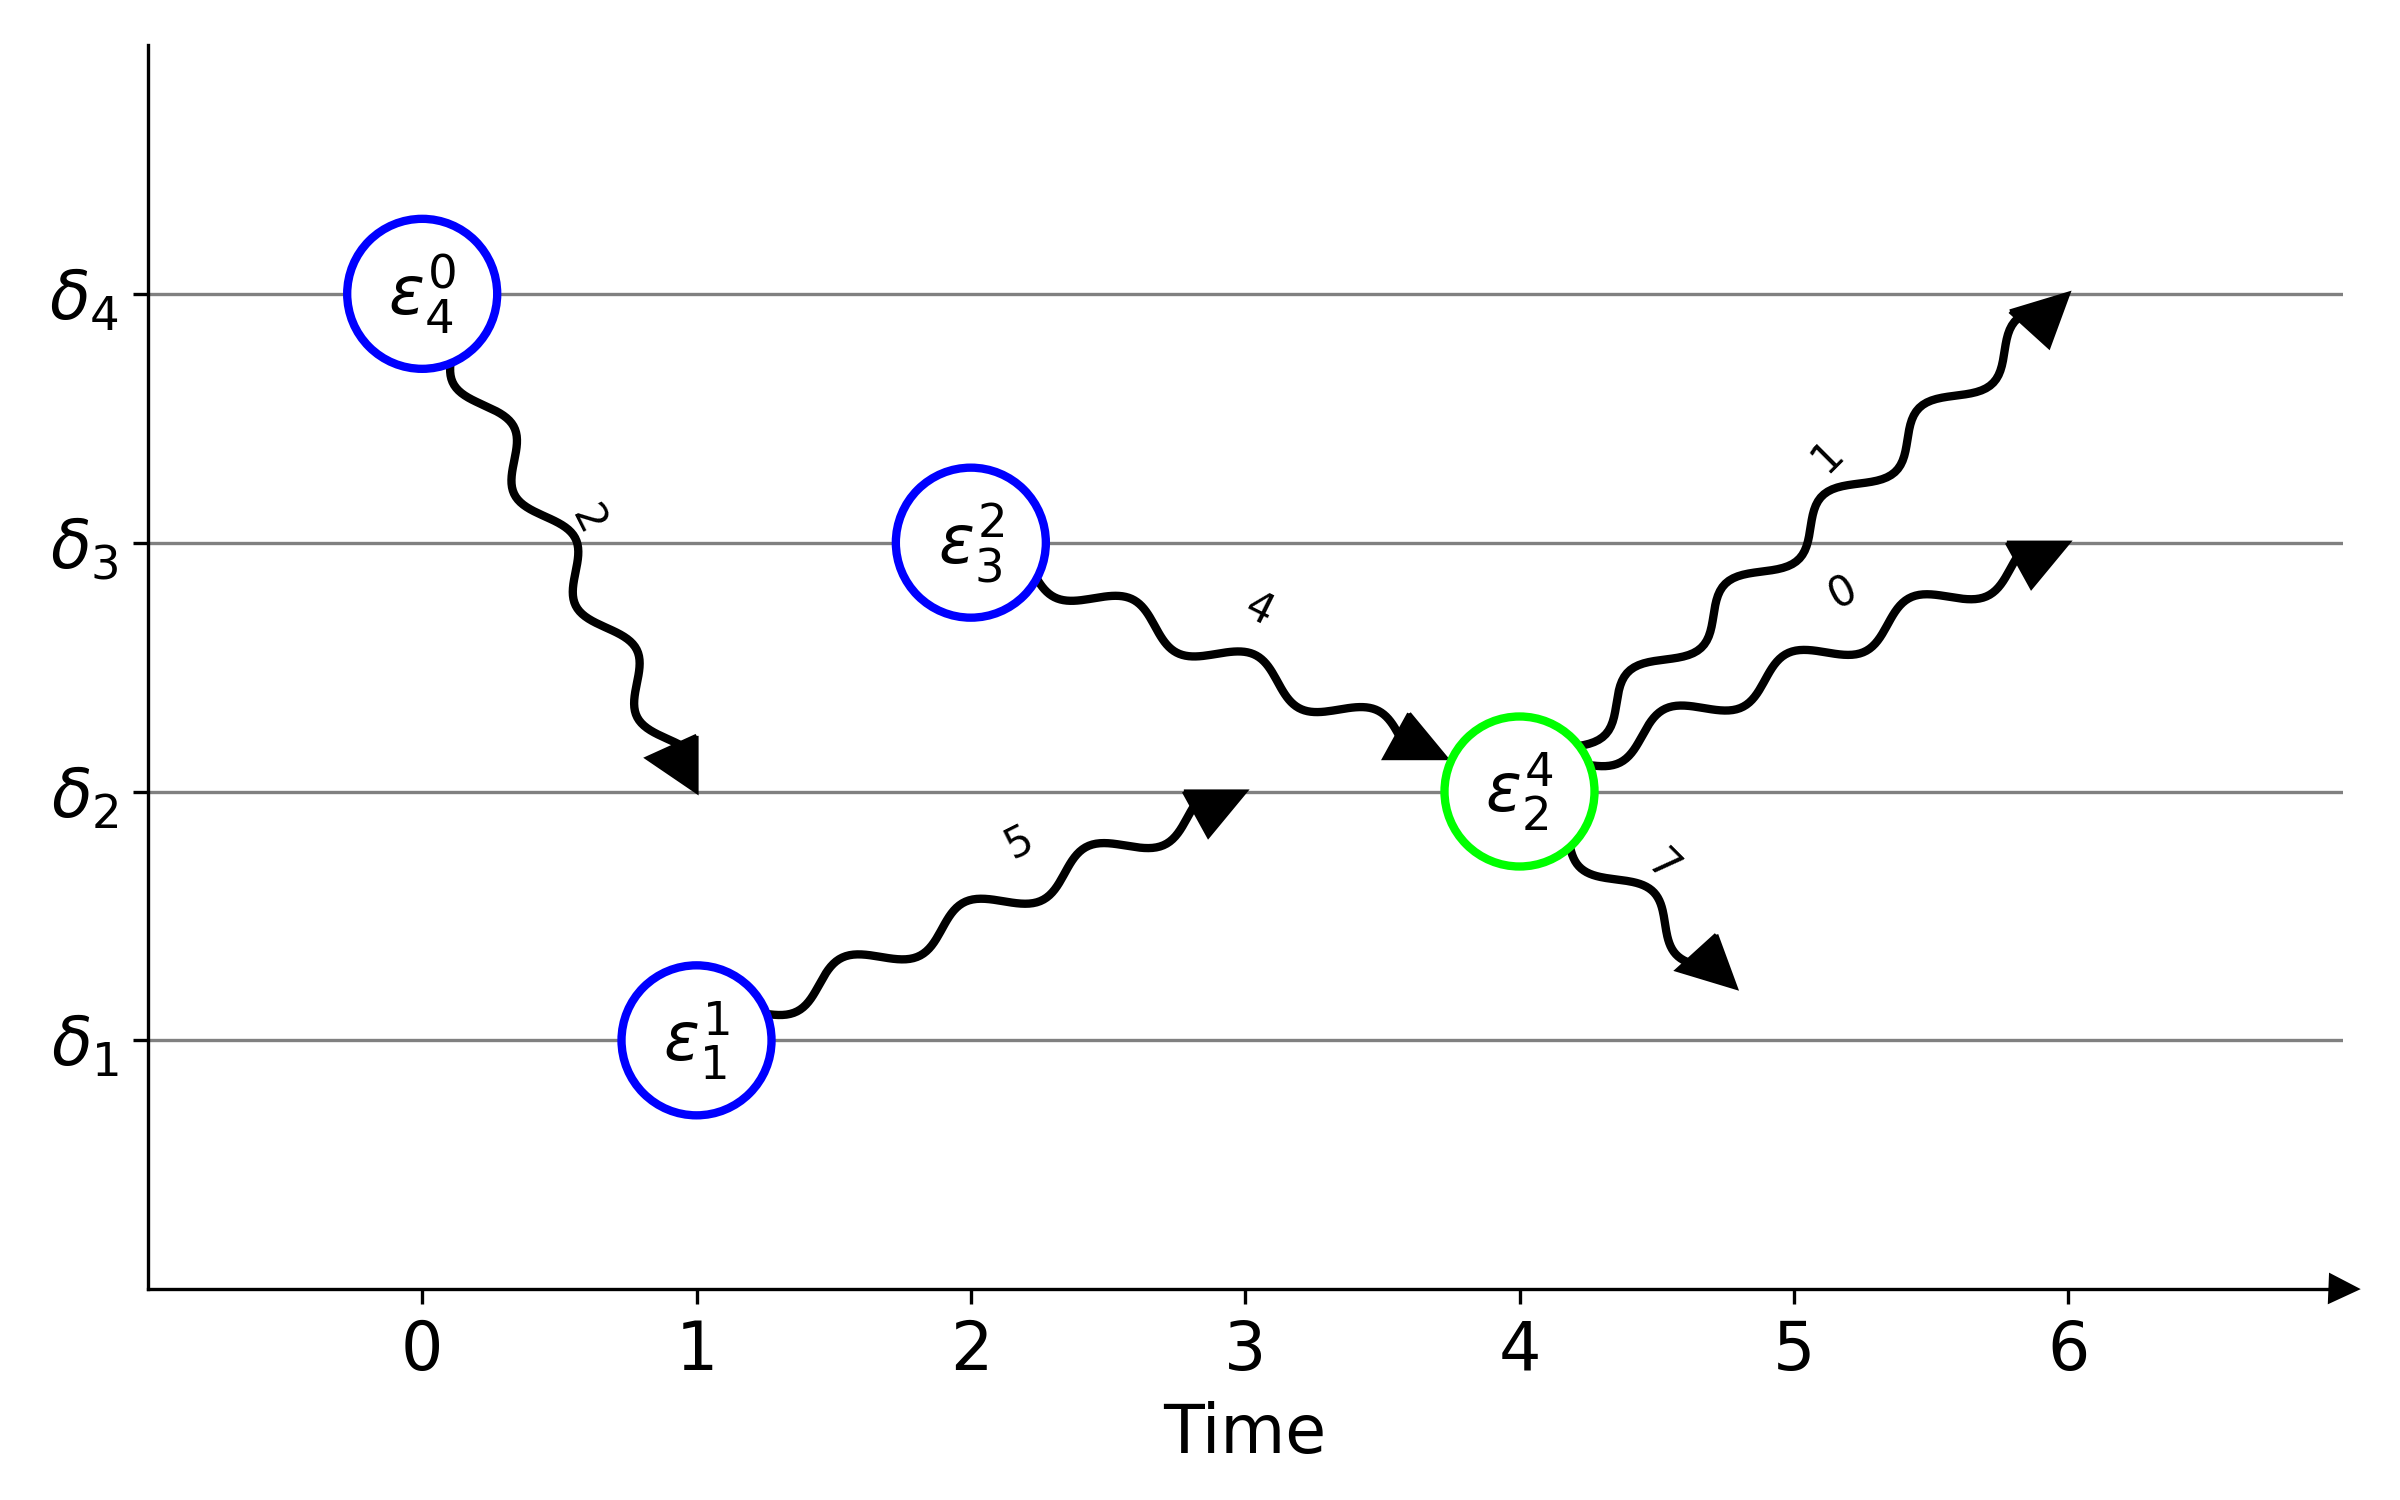
\includegraphics[width=.8\linewidth]{figures/nvalues-example.png}
    \caption{\ac{XC} system model, from the point of view of the wake-up event $\epsilon_2^4$ pictured in green.}
    \label{fig:xc-nvalues-exampke}
\end{figure}

\paragraph{Additional built-in operations} on nvalues are $self(\underline{\mathbf{w}} : \underline{A}) : A$ which returns the local value $\underline{\mathbf{w}}(\delta)$ for the self device $\delta$, and $updateSelf(\underline\mathbf{w} : \underline{A}, l : A) : \underline{A}$ which returns a new nvalue with the same content of $\underline{\mathbf{w}}$ but with the value for the self device replaced by $l$\cite{xc}.
%
Given the built-in function $uid$ that returns the device identifier of the self device, the following property holds: $self(\underline{\mathbf{w}}) = \underline{\mathbf{w}}(uid)$.
%
The complete syntax for \ac{XC} is available in the original paper\cite[p. 4]{xc}.

\subsection{The \texttt{exchange} primitive}

The following description is largely based on the original paper for \ac{XC}\cite{xc}.
%
In \ac{XC}, the only communication primitive is the function $exchange(e_i, (\underline{\mathbf{n}}) \Rightarrow \mathbf{return} e_r \mathbf{send} e_s)$, which is defined using syntactic sugar and translates to $exchange(e_i, (\underline{\mathbf{n}}) \Rightarrow (e_r, e_s))$.
%
The evaluation of the primitive follows three steps:
\begin{enumerate}
    \item the device evaluates expression $e_i$ to obtain the \textit{initial} local value $l_i$;
    \item 
\end{enumerate}

\subsection{Alignment}

\section{Scala 3}\label{chap:background->sec:scala3}
